\section{Age-Period-Cohort models}\label{section:Age-period-cohort-models}
Age-period-cohort (APC) models analyse incidence, morbidity, or prevalence rates of diseases or conditions of interest in a temporal fashion by stratifying the observations by age group and observation period \citep{APC-OLD, APC-OLD-2, APC-OLD-3}. Age simply refers to the age of the observed participants at a certain point in time (i.e., period). Consequently, knowing the age of observed participants along with the period of observation, we obtain a perfect linear relationship to determine the birth cohorts of the observed participants, giving us the final cohort term of the model. A major consideration with the APC model lies in selecting the method to remedy the infamous problem of identifiability of the temporal effects \citep{APC-wakefield}. The family of APC models have become prominent in temporal analyses in recent decades, and variants have been proposed to remedy this problem in both frequentist \citep{Rosenberg2023} and Bayesian frameworks \citep{berzuini1993bayesian,berzuini1994bayesian}, each carrying their own advantages and disadvantages. For the application of the APC model in this thesis, we stick to the Bayesian framework of APC models \citep{APC-Bayesian-Yang,APC-Bayesian-Held}, the implications of which are elaborated upon in Section \ref{section:BayesianInference}. The multivariate extension of the APC model, the multivariate APC (MAPC) model \citep{hansell2003copd, jacobsen2004women}, facilitates stratification by factors such as geographic region, income, and in our case, level of attained education. Incorporating several strata into the model entails some additional considerations in the inference of the model, but also provides remedies to the identifiability problem \citep{APC-Bayesian-Andrea}.

In this section, we first provide basic intuition on temporal analyses and what they measure in Section \ref{section:lexis}, before introducing the APC model in its simplest univariate form in Section \ref{section:univariateAPC}. The extension from the univariate APC model to the multivariate APC model then follows in Section \ref{section:multivariate} and the methods of cross-strata inference in the multivariate APC in Section \ref{section:APC-inference}.

\subsection{The Lexis diagram}
\label{section:lexis}
In the application of APC models, the observed data, typically mortality, prevalence, or incidence rates, are represented by the Lexis diagram \citep{Lexis,Lexis2}. The Lexis diagram is a two-dimensional tabulated format for graphical representation of the data, in which the temporal indices "age" and "period" make up the vertical and horizontal axes, respectively. The axes are divided into discrete intervals, typically by calendar years, meaning each interval on the age axis makes up a compartment with each interval on the period axis. Each compartment refers to a group of participants with a certain age at a certain point in time (period). The compartments are filled with information pertaining to the mortality, prevalence, or incidence of a disease or condition, consequently stratifying the data by age and period. As the birth cohort is identifiable by the age and period, it is consequently represented along the diagonal of the tabular format. An example using toy-data to illustrate the Lexis diagram is shown in Figure \ref{figure:Lexis}. The data shown here could represent the number or rate of participants with a disease or condition, such as back pain.

\begin{figure}[!ht]
    \centering
    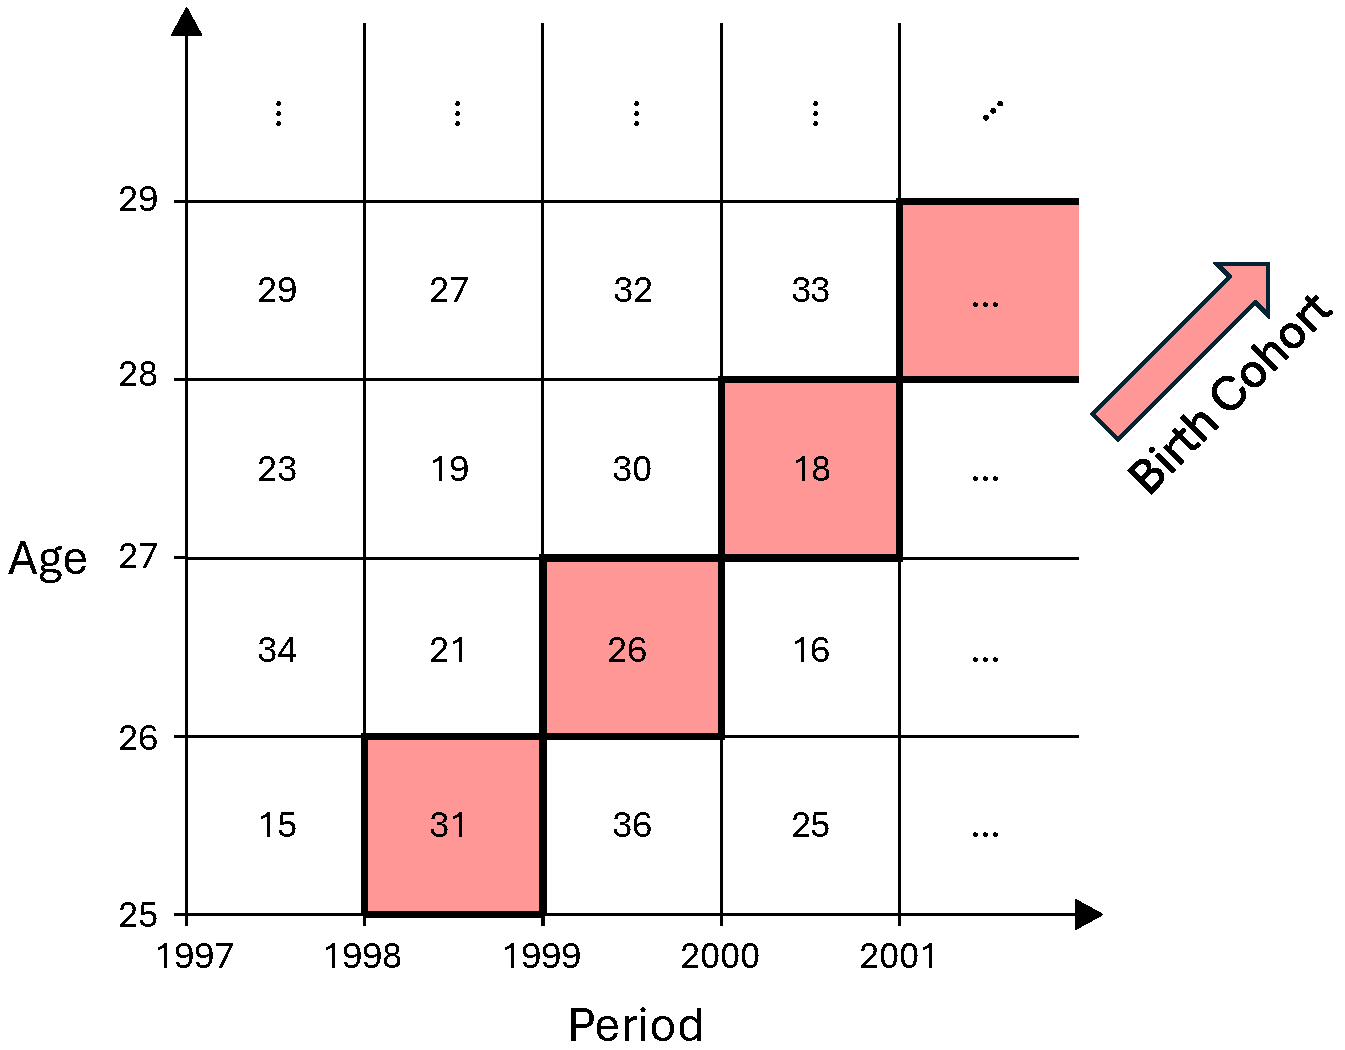
\includegraphics[width = 0.8\textwidth]{./Figures/Lexis.pdf}
    \vspace{-0.2cm}
    \caption{Lexis diagram for example data, such as prevalence of a disease or condition (back pain, in our study). On the axes are age groups and periods with an equal interval length of one year. The cohorts are represented along the diagonals, illustrating the linear dependence between the temporal indices. Marked in red is the example 1998 birth cohort.}
    \label{figure:Lexis}
\end{figure}

%Interpretation of the temporal scales
The temporal inference of the APC model is based on observations of incidences on the three different temporal scales of age, period, and cohort, and stems from proposed methods to analyse data in the format of the Lexis diagram. Though the analysis is performed with respect to time on different scales, it is important to recognize that time itself is not the cause of disease, but rather it represents a way to measure exposure of other factors that operate with time \citep{berzuini1994bayesian}. The ways that these external factors operate and affect the population may be different and difficult to measure, and each of the temporal scales captures different aspects and effects of these factors. Age as a temporal scale is a good substitution for cumulative exposure. As a person grows older, the continued exposure to factors that may cause a disease accumulates, heightening the risk of contracting the disease or condition. Meanwhile, for measuring factors applying to everyone at a certain point in time, the period as a temporal scale is useful. This temporal scale captures shocks, such as sudden outbreaks or major scale events (war, natural disaster, etc.), carrying consequences for the disease or condition of interest. Finally, examining the data using cohorts as a temporal scale helps identify the impact of factors that has changed gradually over time and generations, such as the evolving health habits in the general population or living conditions.

\subsection{The univariate age-period-cohort model}\label{section:univariateAPC}
First, let us define the univariate APC model mathematically. Let $n_{ij}$ denote the number of participants at risk in age group $i$ $(i = 1,...,I)$, with observations taken in period $j$ $(j = 1,...,J)$, stemming from the birth cohort $k$ $(k=1,..,K)$. As the index $k$ may always be derived from $i$ and $j$, it is consequently omitted from notation when accompanied by $i$ and $j$. Furthermore, we assume that the discrete number of observed incidents $y_{ij}$ follows a binomial distribution with the probability of back pain $\pi_{ij}$ and number of trials $n_{ij}$, corresponding to the size of the respective group. Since our application examines a dichotomous outcome noting observations of both presence and absence of back pain, a binomial model is suitable. With the assumption of independent observations, the joint likelihood may be written as a product of binomial terms. In applications, several discrete probability distributions such as the Poisson (as in the original formulation by \cite{clayton1987models}) and negative binomial distributions may be used, though we only consider the case of binomial likelihood (for the application at hand). With these assumptions, the univariate APC model models the log-odds probability of back pain $\pi_{ij}$ as a linear predictor with an overall intercept $\mu$, age effects $\theta_i$, period effects $\phi_j$, and cohort effects $\psi_k$. That is,
\begin{equation}
    \log\left(\frac{\pi_{ij}}{1-\pi_{ij}}\right) = \mu + \theta_i + \phi_j +\psi_k.
\end{equation} 
To ensure identifiability of the intercept, sum-to-zero constraints are typically imposed on $\pmb \theta$, $\pmb \phi$ and $\pmb \psi$. An interesting area of discussion for this model revolves around the perfect linear combinations between the three temporal indices, since the cohort index is directly derived from the age and period index as $k = I-i+j$. Due to the linear dependence of the cohort index on the age and period indices, a second constraint is required to identify the separate contributions of the three temporal effects. For equally-spaced data, this is evident as changes in linear trends only cause a change in the estimated set of parameters all while keeping the linear predictor the same \citep{riebler2010multivariate}. As a consequence, only non-linear trends, such as second differences, are identifiable \citep{clayton1987models}. Particular considerations occur when age and period are defined on different time grids, with different granularity (i.e. month and year). Since we will be using the same granularity for all our temporal indices, these considerations are not covered here, though  further details are provided by \cite{riebler2010multivariate}.

%Resolutions to the identifiability problem
In frequentist settings, the additional constraint has been imposed in several ways with many proposed remedies. These remedies include fixing one temporal effect to zero, equating two effects at one time point \citep{fienberg1979identification}, including additional covariates, or introducing penalty functions to be minimized \citep{osmond1982age}. While these remedies ensure identifiable effects, they are also only identifiable in the context of the imposed constraint, and are therefore difficult to interpret without expert knowledge. In our case, we stick to the Bayesian framework to provide model fit, and make use of the upcoming multivariate version of the APC model to remedy the problem. 

\subsection{The multivariate age-period-cohort (MAPC) model}
\label{section:multivariate}
In several applications, such as ours, it is desirable to compare temporal trends for different strata defined in terms of education, health outcome, sex, activity, or some other factor. While it is possible to use separate APC models for each stratum, especially when prediction is of interest, the issue of identifiability makes comparison between the strata difficult and unintuitive. For these contexts, it is better to use a multivariate APC model to investigate heterogeneous temporal trends. This requires data sets over the same periods and age groups for each stratum that we wish to include in the model. In terms of the Lexis diagrams introduced in Section \ref{section:lexis}, this equates to having multiple diagrams, one for each stratum. For example, one may consider that each compartment of the diagram has observations for each stratum. The multivariate APC models captures the heterogeneous time trends across the different strata, and for comparable strata, the similar factors are likely to work on the same time scales. In applications, it is useful to consider whether an effect should be shared across the different strata. For instance, consider a model where the age effect is shared across the different strata. Following the extension from the univariate APC model to the multivariate APC model by \cite{riebler2010multivariate}, this model would read
\begin{equation}
    y_{ijr}\mid \pi_{ijr} \sim \text{Binomial}(\pi_{ijr}, n_{ijr}),
    \label{eqn:likelihood-MAPC}
\end{equation}
where $y_{ijr}$ is the observed number of cases for age group $i$ in period $j$ from cohort $k$ (omitted as it depends on $i$ and $j$) following strata $r$ ($r=1,...,R$), and $n_{ijr}$ is the size of the group. The linear predictor for the log-odds of $\pi_{ijr}$ is then
\begin{equation}
    \log\left(\frac{\pi_{ijr}}{1-\pi_{ijr}}\right) = \mu_r + \theta_i + \phi_{jr} + \psi_{kr},
    \label{eqn:linear-predictor}
\end{equation}
where $\mu_r$ is the stratum-specific intercept for stratum $r$, $\theta_i$ is the 
age effect shared across each stratum, and $\phi_{ir}$ is the stratum-specific period effect and $\psi_{kr}$ is the stratum-specific cohort effect. To ensure identifiability of the stratum-specific intercepts, sum-to-zero constraints are imposed on the age, period, and cohort effects. That is
\begin{equation}
    \sum_{i}\theta_i=0,\quad \sum_j\phi_{jr}=0\quad \text{and}\quad \sum_k\psi_{kr}=0\;\; \text{for all } r = 1,...,R.
\end{equation}
Adapting this model structure for different shared effects is simple, though some care has to be taken when selecting a model for a specific analysis. If the age effect across strata is of inferential importance, then the model should naturally include a stratum-specific effect over age. Similarly, if period or cohorts are of specific interest, then a different combination of shared and stratum-specific effects should be considered. Should no combination be preferred a priori, then model selection may be used to settle on a model. Note also that the multivariate formulation of the APC model adapts the same issues regarding identifiability as the univariate. The remedy used in our application is presented in Section \ref{section:APC-inference}.

For future reference of different specifications of shared and stratum-specific effects in the multivariate APC model, the abbreviation APC will be capitalized based on which effects are shared and which are stratum-specific. Effects shared across strata are shown by uppercase letters (A, P, C) and for effects that are stratum-specific we use lowercase letters (a, p, c). For instance, the above model with shared age effect, but stratum-specific period and cohort effects would be abbreviated as the Apc model. 

\subsection{Cross strata inference with MAPC models}
\label{section:APC-inference}
A major benefit of using the multivariate APC model instead of several univariate models is that differences in effects across strata become identifiable \citep{APC-Bayesian-Andrea}. While the MAPC model inherits the same issues of identifiability as the univariate APC model, the linear predictor remains identifiable, allowing differences in the linear predictor across strata to be identifiable. To elaborate, the issue in APC models of all kinds is that the age, period, and cohort effects are not identifiable by themselves, but the sum of the parts is. Consequently, by examining the cross-strata differences of these sums, we arrive at methods of inference that are identifiable and intuitive. Examining the cross strata differences between each pair of strata is unadvised, since there are many pairs to consider, thus making interpretation difficult. Rather, it is common to analyse differences with respect to only one stratum, which is chosen subjectively to the application at hand. In our case, BA+ level of attained education is chosen, since this group is better represented in terms of sample size, and experienced better health outcomes. Consequently, we want to identify health disparities compared to the healthiest group. Moreover, due to the imposed sum-to-zero constraints on each temporal effect, shared effects cancel out, leaving only the difference in the effects varying across strata. A slight limitation to this is that at least one effect has to be shared across strata for these differences to be identifiable. To derive our methods of inference for cross strata differences, we look to the proposed methods of \cite{APC-Bayesian-Andrea}.

\subsubsubsection*{Only one stratum-specific effect}
\vspace{-0.2cm}
To acquire some understanding and intuition on the inference obtained by investigating cross strata differences, let us consider the simplest case with only one stratum-specific effect. To this end, consider an aPC model with the linear predictor
\begin{align}
    \log\left({\frac{\pi_{ijr}}{1-\pi_{ijr}}}\right) = \mu_r + \theta_{ir} + \phi_j + \psi_k,
\end{align}
with corresponding sum-to-zero constraints on each of the temporal effects. Now, let us consider two strata $r_1$ and $r_2$, each with $I$ age groups over $J$ periods, giving rise to $K$ cohorts. As mentioned earlier, we have to make a subjective choice of what stratum to compare against. For two strata, this choice may not be as important, but it might be important to consider what makes sense for several available strata. Let us choose $r_1$ as the baseline stratum to compare against, then we may for each $i$, $j$ and $k$ compute the cross strata difference, denoted $\Delta_{i}$, as the difference in the linear predictor:
\begin{align}
    \begin{split}
    \Delta_{i} &= \mu_{r_2} + \theta_{ir_2} + \phi_{j} + \psi_{k} - (\mu_{r_1} + \theta_{ir_1} + \phi_{j} + \psi_{k})\\
    & = \mu_{r_2} - \mu_{r_1 } + \theta_{ir_2} - \theta_{ir_1}.
    \end{split}
    \label{eqn:deltai}
\end{align}
Notice that the shared effects $\phi_j$ and $\psi_k$ cancel out, leaving only terms dependent on age group $i$ and strata. Since Equation \eqref{eqn:deltai} is the difference in the linear predictor, we may also express this difference in terms of the log-odds since
\begin{align}
    \begin{split}
    \Delta_{i} &= \log\left(\frac{\pi_{ijr_2}}{1-\pi_{ijr_2}} \right) - \log\left(\frac{\pi_{ijr_1}}{1-\pi_{ijr_1}} \right)\\ &= \log\left(\frac{\frac{\pi_{ijr_2}}{1-\pi_{ijr_2}}}{\frac{\pi_{ijr_1}}{1-\pi_{ijr_1}}}\right)=\log\left(\text{OR}_i\right),
    \end{split}
    \label{eqn:deltailog}
\end{align}
where $\text{OR}_i$ denotes the odds ratio of back pain in each stratum. Notice that since the difference in the linear predictors in Equation \eqref{eqn:deltai} does not depend on the temporal indices $j$ and $k$, the odds ratio $\text{OR}_i$ only depends on $i$. Putting Equations \eqref{eqn:deltai} and \eqref{eqn:deltailog} together, we may express the odds ratio as
\begin{align}
    \text{OR}_i = \exp\{\mu_{r_2} - \mu_{r_1 } + \theta_{ir_2} - \theta_{ir_1}\}.
    \label{eqn:ORi}
\end{align}
In our application, we obtain (from our model) the values of Equation \eqref{eqn:deltai}, which we then transform into Equation \eqref{eqn:ORi} for interpretation. In the case of only one stratum-specific effect, the interpretation of the odds ratio is simple and intuitive. The interpretation is discussed after presenting the derivation when the model has two stratum-specific effects.

\subsubsubsection*{Two stratum-specific effects}
\vspace{-0.2cm}
As we investigate cross strata differences in models with two stratum-specific effects, the interpretation of the cross strata differences becomes somewhat more complex. To illustrate, let us consider the example Apc model represented by Equations \eqref{eqn:likelihood-MAPC} and \eqref{eqn:linear-predictor}. Let us once again consider the two strata $r_1$ and $r_2$, with $I$ age groups over $J$ periods, giving rise to $K$ cohorts, and let us choose $r_1$ as the baseline stratum to compare against. This time, our cross strata difference will depend on two temporal indices, namely $j$ and $k$. The cross strata difference, therefore denoted $\Delta_{jk}$, is consequently expressed as
\begin{align}
    \begin{split}
    \Delta_{jk} &= \mu_{r_2} + \theta_i + \phi_{jr_2} + \psi_{kr_2} - (\mu_{r_1} + \theta_i + \phi_{jr_1} + \psi_{kr_1})\\
    & = \mu_{r_2} - \mu_{r_1 } + \phi_{jr_2} - \phi_{jr_1} + \psi_{kr_2} - \psi_{kr_1}.
    \end{split}
    \label{eqn:deltajk}
\end{align}
Notice that the shared effect $\theta_i$ cancels out. As the cross strata difference now depends on two temporal indices, we proceed by averaging over each temporal index separately, yielding two estimates, each only dependent on one temporal index. Let us define the cohort cross strata difference, denoted $\Tilde{\Delta}_k$, by averaging Equation \eqref{eqn:deltajk} over $j$ as
\begin{align}
    \Tilde{\Delta}_{k} & = \frac{1}{J}\sum_{j=1}^J \Delta_{jk} = \mu_{r_2} - \mu_{r_1 } + \psi_{kr_2} - \psi_{kr_1},
    \label{eqn:deltak}
\end{align}
where the terms $\phi_{jr_1}$ and $\phi_{jr_2}$ cancel out due to the imposed sum-to-zero constraints. The corresponding definition for the second cross strata difference, $\Tilde{\Delta}_j$, is made by averaging over the other temporal index $k$ instead. Moreover, $\Delta_{jk}$, in Equation \eqref{eqn:deltajk} may also be expressed using the left-hand side of the linear predictor in Equation \eqref{eqn:linear-predictor} as
\begin{align}
    \begin{split}
    \Delta_{jk} &= \log\left(\frac{\pi_{ijr_2}}{1-\pi_{ijr_2}} \right) - \log\left(\frac{\pi_{ijr_1}}{1-\pi_{ijr_1}} \right)\\  &= \log\left(\frac{\frac{\pi_{ijr_2}}{1-\pi_{ijr_2}}}{\frac{\pi_{ijr_1}}{1-\pi_{ijr_1}}}\right) = \log\left(\text{OR}_{jk}\right).
    \end{split}
    \label{eqn:deltajk2}
\end{align}
Combining Equations \eqref{eqn:deltak} and \eqref{eqn:deltajk2}, we see that the cross strata difference may be expressed as
\begin{align}
    \begin{split}
    \Tilde{\Delta}_{k} &= \frac{1}{J}\sum_{j=1}^J \Delta_{jk} = \frac{1}{J}\sum_{j=1}^J\log\left(\text{OR}_{jk}\right)\\ 
    & =\frac{1}{J}\log\left(\prod_{j=1}^J\text{OR}_{jk}\right) = \log\left(\left[\prod_{j=1}^J\text{OR}_{jk} \right]^\frac{1}{J} \right),         
    \end{split}
\end{align}
and therefore,
\begin{align}
    \begin{split}
    \left(\prod_{j=1}^J\text{OR}_{jk} \right)^\frac{1}{J} = \exp\{\mu_{r_2} - \mu_{r_1 } + \psi_{kr_2} - \psi_{kr_1}\},
    \end{split}
    \label{eqn:ORjk}
\end{align}
which we identify as the geometric mean of the odds ratio in cohort $k$ with respect to the periods $j$. By use of our models we may compute the right-hand side of Equation \eqref{eqn:ORjk}, which for each cohort $k$ gives us estimates to be interpreted as geometric mean odds ratios with respect to the period $j$. For the example model used here, we would obtain the geometric mean of the odds ratio in period $j$ with respect to the cohorts $k$ in a similar manner. In models with two stratum-specific effects, the geometric mean of the odds ratio presented over one temporal index will always be the geometric mean with respect to the other temporal index. As a consequence for future reference, when using a model with two stratum-specific effects, we will be referring to the geometric mean of odds ratios simply as odds ratios, neglecting the index of which the mean is with respect to.

In either case, whether the model has one or two stratum-specific effects, the exponential of the cross strata differences is still interpreted as a ratio of odds. Our choice of baseline stratum entails that, for the age group, period, or cohort at hand, the odds in the denominator of the ratio corresponds to the odds of having back pain in participants with BA+ level of attained education. The alternative stratum, with odds in the numerator of the ratio, is for participants with the alternative level of attained education, in the same age group, period or cohort. Therefore, if the odds ratios are observed to be grater than one, it signals a greater risk in the age group, period, or cohort with the alternative level of attained education, compared to the corresponding group with the baseline level of attained education. Conversely, if the observed odds ratio is smaller than one, then it signals that the risk is greater in participants with the baseline level of education rather than the alternative. A frequentist approach to comparing effects across different strata is presented by \cite{Rosenberg2023}.

By our Bayesian implementation (to be detailed in Section \ref{section:application1:specification}), we obtain estimates of the log-odds ratios as Gaussian distributions over the relevant temporal indices of the model, allowing us to quantify our uncertainty of the model estimates, typically taken as the mean or median of the distribution.





